\documentclass[border=3pt]{standalone}
\usepackage{tikz}
\usetikzlibrary{arrows.meta,calc}
\tikzset{pin/.style={-{Stealth[length=5pt]}},
  blk/.style={draw, thick, minimum width=20mm, minimum height=22mm, font=\sffamily}}
\begin{document}
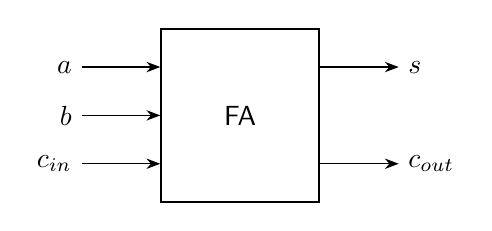
\begin{tikzpicture}[font=\sffamily]
  \node[blk] (fa) {FA};
  % inputs on the left
  \draw[pin] ($(fa.north west)+(-10mm,-5mm)$) node[left]{$a$} -- ($(fa.north west)+(0,-5mm)$);
  \draw[pin] ($(fa.west)+(-10mm,0)$) node[left]{$b$} -- (fa.west);
  \draw[pin] ($(fa.south west)+(-10mm,5mm)$) node[left]{$c_{in}$} -- ($(fa.south west)+(0,5mm)$);
  % outputs on the right
  \draw[pin] ($(fa.north east)+(0,-5mm)$) -- ++(10mm,0) node[right]{$s$};
  \draw[pin] ($(fa.south east)+(0,5mm)$) -- ++(10mm,0) node[right]{$c_{out}$};
\end{tikzpicture}
\end{document}
